\documentclass{standalone}

\usepackage{tikz}
\usetikzlibrary{shapes, arrows}
\usetikzlibrary{calc}

\tikzset{
%
data/.style={
% The shape:
rectangle,
% The size:
minimum size=6mm,
% The border:
very thick,
draw=black!80,
% fill
fill=gray!20
},%
%
preprocess/.style={
% The shape:
trapezium, 
trapezium left angle=60, 
trapezium right angle=-60,
% The size:
minimum size=6mm,
% The border:
very thick,
draw=black!80,
% fill
fill=gray!20
},%
%
gams/.style={
% The shape:
ellipse,
% The size:
minimum size=6mm,
% The border:
very thick,
draw=black!80,
% fill
fill=gray!20
},%
}

\begin{document}

\newcommand{\mltext}[2]{\begin{tabular}{c} #1 \\ #2 \end{tabular}}

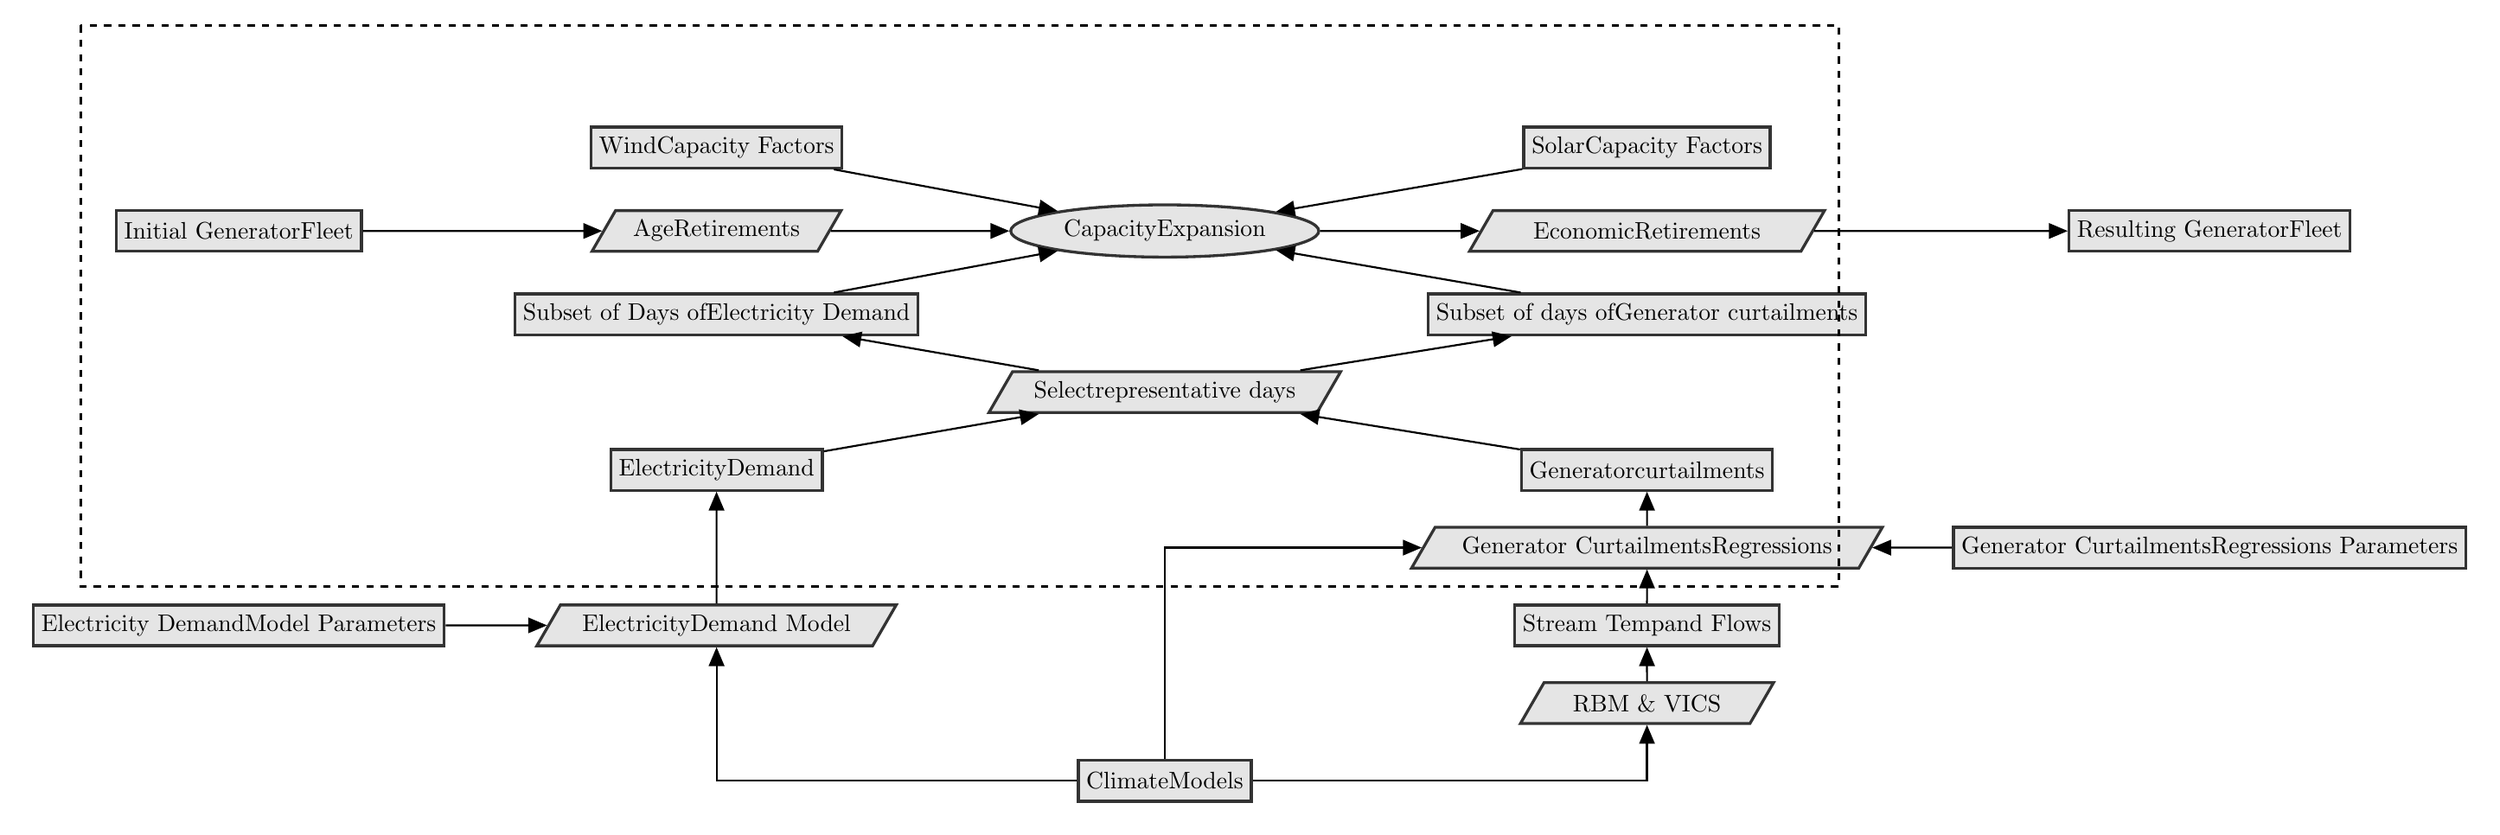
\begin{tikzpicture}
\matrix[row sep=5mm,column sep=10mm] {
% first row
 & \node [data]  (windcf) {\mltext{Wind}{Capacity Factors}}; & & \node [data]  (solarcf) {\mltext{Solar}{Capacity Factors}}; \\
% 2nd row
\node [data] (initial fleet) {\mltext{Initial Generator}{Fleet}};  &
\node [preprocess]  (pre retire) {\mltext{Age}{Retirements}}; &
\node [gams]  (ce) {\mltext{Capacity}{Expansion}}; &
\node [preprocess]  (post retire) {\mltext{Economic}{Retirements}}; & 
\node [data] (final fleet) {\mltext{Resulting Generator}{Fleet}};
\\
% third row
&  \node [data] (demand sub) {\mltext{Subset of Days of}{Electricity Demand}}; & & \node [data] (curtail sub) {\mltext{Subset of days of}{Generator curtailments}};\\
% fourth rows
&& \node [preprocess] (rep days) {\mltext{Select}{representative days}}; &\\
% 5th rows
&  \node [data] (demand) {\mltext{Electricity}{Demand}}; & & \node [data] (curtail) {\mltext{Generator}{curtailments}};\\
% 6th rows
&  & & \node [preprocess] (curtailregression) {\mltext{Generator Curtailments}{Regressions}}; & \node [data] (curtailregressionparam) {\mltext{Generator Curtailments}{Regressions Parameters}};\\
% 7th rows
\node [data] (demandmodelparam) {\mltext{Electricity Demand}{Model Parameters}}; & \node [preprocess] (demandmodel) {\mltext{Electricity}{Demand Model}};  & & \node [data] (waterdata) {\mltext{Stream Temp}{and Flows}};\\
% 8th rows
& & & \node [preprocess] (uw) {\mltext{RBM \& }{VICS}};\\
% 9th rows
& & \node [data] (gcms) {\mltext{Climate}{Models}}; & \\
};
%
%
% Edges
\path[-triangle 45, thick]  	(windcf) edge (ce)
					(solarcf) edge (ce)				
					(initial fleet) edge (pre retire) 
					(pre retire) edge (ce)
					(ce) edge (post retire)
					(post retire) edge (final fleet)
					(demand sub) edge (ce)
					(curtail sub) edge (ce)				
					(rep days) edge (demand sub)
					(rep days) edge (curtail sub)				
					(demand) edge (rep days)
					(curtail) edge (rep days)
					(demandmodel) edge (demand)
					(curtailregression) edge (curtail)
					(uw) edge (waterdata)
					(waterdata) edge (curtailregression)
					(curtailregressionparam) edge (curtailregression)
					(demandmodelparam) edge (demandmodel);
					
\draw[->,-triangle 45, thick]	(gcms.west) -| (demandmodel.south);
\draw[->,-triangle 45, thick]	(gcms.north) |- (curtailregression.west);
\draw[->,-triangle 45, thick]	(gcms.east) -| (uw.south);


% rectangle of our model
\draw[very thick, dashed]     ($(initial fleet.north west)+(-0.5,2.7)$) rectangle ($(curtailregression.south east)+(2.5,-0.25)$);

\end{tikzpicture}

\end{document}  